\chapter{Description des composants}

L'architecture qui sera détaillée par la suite se limitera à notre partie, a
savoir les composants définis par les entités clientWeb et ServeurWeb : \\

\begin{figure}[H]
\begin{center}
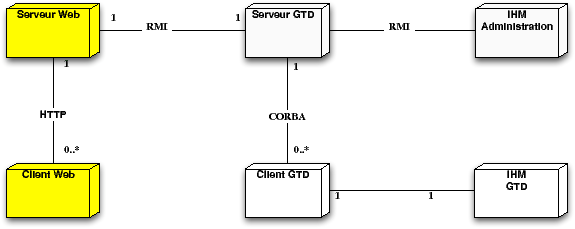
\includegraphics[scale=0.9]{livrable3/images/archi.png}
\caption{Architecture Générale - Entités modélisées}
\end{center}
\end{figure}


\section{Liste des composants}

\begin{figure}[H]
\begin{center}
\includegraphics[scale=0.7]{livrable3/images/composants2.png}
\caption{Architecture Générale - Diagramme de composants}
\end{center}
\end{figure}

L'application est composée des composants suivants :
\begin{itemize}
  \item WebClient
  \item ConnectionManager
  \item DataManager
  \item ProcessManager
\end{itemize}

Chacun d'eux est décrit ci-dessous.


\section{Composant ClientWeb}
L'utilisateur se connectera au serveur GTD à l'aide du composant WebClient. Ce
composant est une RIA (Rich Internet Application). Le programme initialement écrit en Java sera transformé à l'aide du compilateur GWT en langage Web (javascript, HTML et css). Il permet donc
d'alléger la charge du serveur web : Contrairement à du
jsp qui est exécuté sur le serveur web, celui-ci va être exécuté sur le client.

\medskip

Le composant WebClient va utiliser les interfaces fournies par le
WebServer. Celui-ci est en effet un service, les appels vont donc être réalisés
via RPC (en javascript). GoogleWebToolkit fournit l'ensemble des outils nécessaires à la
réalisation de cette communication.

\section{Composant ConnectionManager}


Ce composant s'occupe de gérer l'ensemble des sessions utilisateurs. 
En effet notre client Web pouvant être utilisé par une multitude de personnes, le composant s'occupe d'assurer 
l'identification vers le serveur GTD et/ou ToodleDo, la connexion entre notre
serveur Web et le serveur GTD et/ou ToodleDo. Lors d'une perte de connexion
entre le client et le serveur Web, il s'occupera d'envoyer une demande de
déconnexion vers le(s) serveur(s).

	\subsection{Gestion des comptes ToodleDo et du serveur GTD}
	L'application fonctionne avec différents serveurs. Ainsi, le choix qui à été fait consiste à regrouper les informations de chaque serveur (login, password) au sein d'un meta-compte. Celui-ci, dispose de son propre login et mot de passe. Il permet à l'utilisateur de saisir un seul couple login mot de passe pour se connecter aux serveurs ToodleDo et GTD. Les informations concernant ses comptes sont stockées localement sur le serveur d'application.

	\subsection{Liaison vers le client}
	La communication avec le client sera effectuée à l'aide de l'interface
	IGTDWebServer. Cette interface expose toutes les méthodes de
	ConnectionManager et ProcessManager. Le WebServer peut grâce à elle,
	rediriger les bons appels de connexion/déconnexion vers le composant
	ConnectionManager, et les appels métiers vers ProcessManager.


	\subsection{Liaison vers DataManager}
	La communication avec le composant DataManager est effectuée par
	l'implémentation des méthodes décrites par l'interface du composant ConnectToServer.
	
	\subsection{Test des connexions et gestion des erreurs}
	Ce composant doit permettre d'indiquer aux autres composants l'état des connexions en temps réel. Pour cela lors de la phase de 
	connexion, il teste la disponibilité des deux serveurs à savoir du serveur GTD
	et de ToodleDo. L'interception des exceptions permettra de modifier l'état des
	connexions à chaque instant. En effet, lorsqu'une exception sera levée de la part du DataManager, il en informera ses observateurs (dont ConnectionManager). Ce dernier mettra alors à jour les données de connexion.


\section{Composant DataManager}


Le composant DataManager va faire le lien entre la couche métier (le composant
ProcessManager) et les serveurs GTD / ToodleDo. Il va donc permettre de répondre
au problématiques suivantes : \\

\begin{itemize}
 \item Permettre la communication entre le ConnectionManager et les serveurs GTD
 et ToodleDo
 \item Permettre de renvoyer à la couche métier les données en provenance du
 serveur GTD et ToodleDo
 \item Permettre la synchronisation du serveur GTD au serveur ToodleDo
 \item Permettre la synchronisation du serveur ToodleDo au serveur GTD\\
\end{itemize}




\subsection{Gestion des serveurs GTD et ToodleDo}

Le composant DataManager doit rendre l'utilisation des
serveurs ToodleDo et GTD transparente pour la couche métier (ProcessManager).
Ainsi, les données envoyées et reçues par celle-ci seront génériques et donc de
niveau métier. Cependant, lors de la transmission des données du DataManager au
serveur GTD et ToodleDo, le DataManager va devoir les adapter au bon format des
serveurs. En effet, un certain nombre de concepts diffèrent d'un serveur à l'autre. 
Par exemple, la notion de notes présente dans le serveur GTD ne l'est pas dans ToodleDo. 
De plus, il faut considérer différents scénarios possibles en cas de problèmes
avec les serveurs :


\subsubsection*{Gestion des connexions}

Comme le montre le diagramme de composant, le DataManager est le seul composant
relié aux serveurs. Il va donc devoir gérer les connexions et les transactions et va faire le lien entre la session utilisateur et les deux serveurs. Les couples login/password associés aux serveurs ne sont pas stockés dans ce composant mais dans le composant ConnectionManager.



\subsubsection*{Le serveur ToodleDo n'est plus disponible}

Si jamais le serveur ToodleDo venait à être indisponible, le DataManager
doit prévenir le composant ProcessManager, qui lui même informera le GUI.
Etant donné que ToodleDo ne dispose pas de toutes les fonctionnalités de GTD,
l'utilisateur ne constatera pas de différence sur la GUI. Une synchronisation
ultérieure sera nécessaire pour conserver une cohérence des données entre le
serveur GTD et ToodleDo.

\subsubsection*{Le serveur GTD n'est plus disponible}
Les fonctionnalités GTD étant plus nombreuses, en cas d'indisponibilité du
serveur GTD, l'affichage des données sera limitée sur la GUI. En effet, les
données, bien que génériques, seront limitées aux fonctionnalités du serveur
ToodleDo. En cas d'indisponibilité des deux serveurs, le Data manager
l'informera au ConnectionManager.

\section{Composant ProcessManager}

Le processManager est le composant dédié au traitement métier de
l'application.Il fait parti du WebServer et intervient une fois que le
 ConnectionManager a établit la connexion à un serveur GTD et/ou ToodleDo.
Son rôle est donc d'effectuer les calculs et vérification. Ses fonctionnalités
sont les suivantes :\\
\begin{itemize}
  \item CRUD Idées
  \item CRUD Tâches
  \item CRUD Projet
  \item CRUD Notes
  \item CRUD Contexte
  \item Vérification des contraintes métier avant chaque opération
  \item Synchronisation des données
\end{itemize}


\subsection*{Couche métier de l'application}
Le ProcessManager contient toute la couche métier de l'application. A un niveau
plus générique, elle correspond au données stockées dans le serveur GTD. Ces
classes seront cependant amenées à 'voyager' entre les composants car elles
seront utilisées comme conteneur de données dans les échanges.

    
\subsection*{Précondition à chaque opération}
Avant chaque opération demandée à la couche métier, il est nécessaire de
vérifier que les modifications pourront être faites sur les serveurs distants.
Pour ce faire, le ProcessManager peut vérifier que la session est utilisable
via l'interface qui la relie au ConnectionManager, à savoir IConnManager.

\subsection*{Execution d'une opération}
Le processManager est le coeur métier de l'application, il se situe donc entre
l'ihm et les données. Il reçoit donc les appels du WebClient, modifie sa
représentation interne des donneés puis demande la modification au DataManager.
Cette chaine d'execution est la même pour chaque opération. En effet,
l'application travaille directement avec les serveur GTD et ToodleDo, il n'est
en effet pas concevable de fournir une application mise à disposition sur un
serveur Web, sans internet. Le mode non connecté n'est donc pas recevable; la
couche données de l'application est donc le serveur GTD ou ToodleDo lui même.

\subsection*{Synchronisation des données}
Le composant processManager permet également d'assurer la synchronisation entre les serveurs GTD et ToodleDo. C'est lui qui prend en charge la mise à jour des données d'un serveur vers l'autre. Pour cela, il va notamment utiliser les dates de modification des entités.

